\chapter{Paper} \label{c:Paper}
In this chapter we will examine the topic of the paper \textit{Stable Neo-Hookean Flesh Simulation} \cite{Smith:2018:SNF:3191713.3180491}. In the interest of understanding the thought process of the authors I will include some of their calculations a bit more detailed. In addition examples and visualisations should help for a better understanding. 

\section{Energy Formulation}
The core goal of the paper was to model deformations for virtual characters that have human-like features. They concentrated on the deformation energy. In order to achieve a convincing result as a first step we need to specify some requirements. For our needs in this case the stability of the energy is important. More precisely we need a hyperelastic energy that is stable in the following four important ways:

\begin{itemize}
\item Inversion stability
\item Reflection stability
\item Rest stability
\item Meta-stability under degeneracy
\end{itemize}

\todoredefined[inline]{
TODO: explain each step
}

\subsection{Previous Work}
Here comes previous work in neo-hookean energy formulation. What is neo-hookean and why do we need it here?
And what is wrong with each one.

\subsection{Stable Neo-Hookean Energy}
Conclude to the energy proposed in the paper.

\section{Energy Analysis}
Calculations and Herleitungen

\subsection{First Piola-Kirchhoff Stress (PK1)}
Explain.

\subsection{The Energy Hessian Terms}
Calculations

\subsection{The Tikhonov, Mu, and Gradient Terms}
Calculations

\subsection{The Volume Hessian}
Calculations
 
\subsection{The Complete Eigensystem}
Calculations

\section{Experiments with the Code}
The authors of the paper \textit{Stable Neo-Hookean Flesh Simulation} \cite{Smith:2018:SNF:3191713.3180491} kindly provided the implementation for an application of their formulated energy. In this code they implemented the stretch test on a cube. The outputs were 26 static images with show the deformation in 25 steps. The parameters the code expects are the two lamé parameters $\mu$ and $\lambda$ and a value for defining the desired resolution the objects should have.

\todoredefined[inline]{
TODO: Explain how the code is implemented in simple words and how the energy is taken in account with the poisson's ratio. Make scheme with input - box / code - output. Do I have to reference code?
}

For starters let us take common values for $\mu$ and $\lambda$. We first start with $\mu = 1.0$, $\lambda = 10.0$ and a resolution of 10.0. For the poisson's ratio we get the value $0.4545$:

\[ \sigma =  \frac{10.0}{2 (10.0 + 1.0)} = 0.4545 \in [-1, 0.5] \]


The following images in figure \ref{fig:stretchtest} show the stretch test with $\mu = 1.0$, $\lambda = 10.0$ and a resolution of 10.0 on a tetrahedral and a hexahedral mesh.

\begin{figure}[!htbp]
	\centering
	\begin{subfigure}[b]{\textwidth}
        \centering
        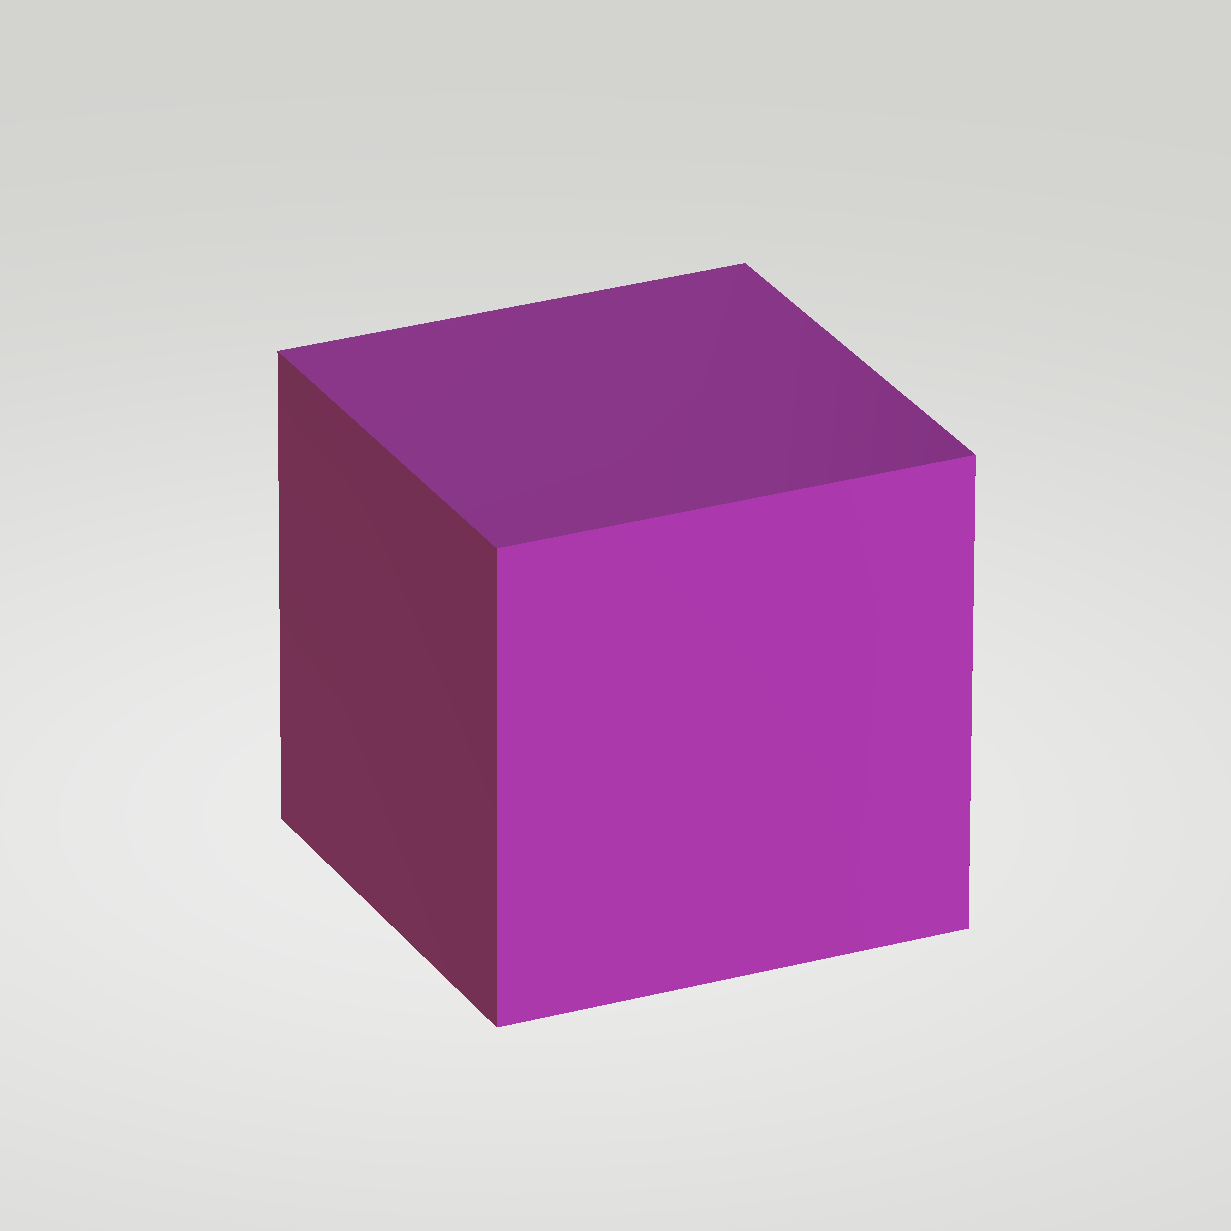
\includegraphics[width=0.24\textwidth]{resources/hexcli_step0.png}
        \hfill
        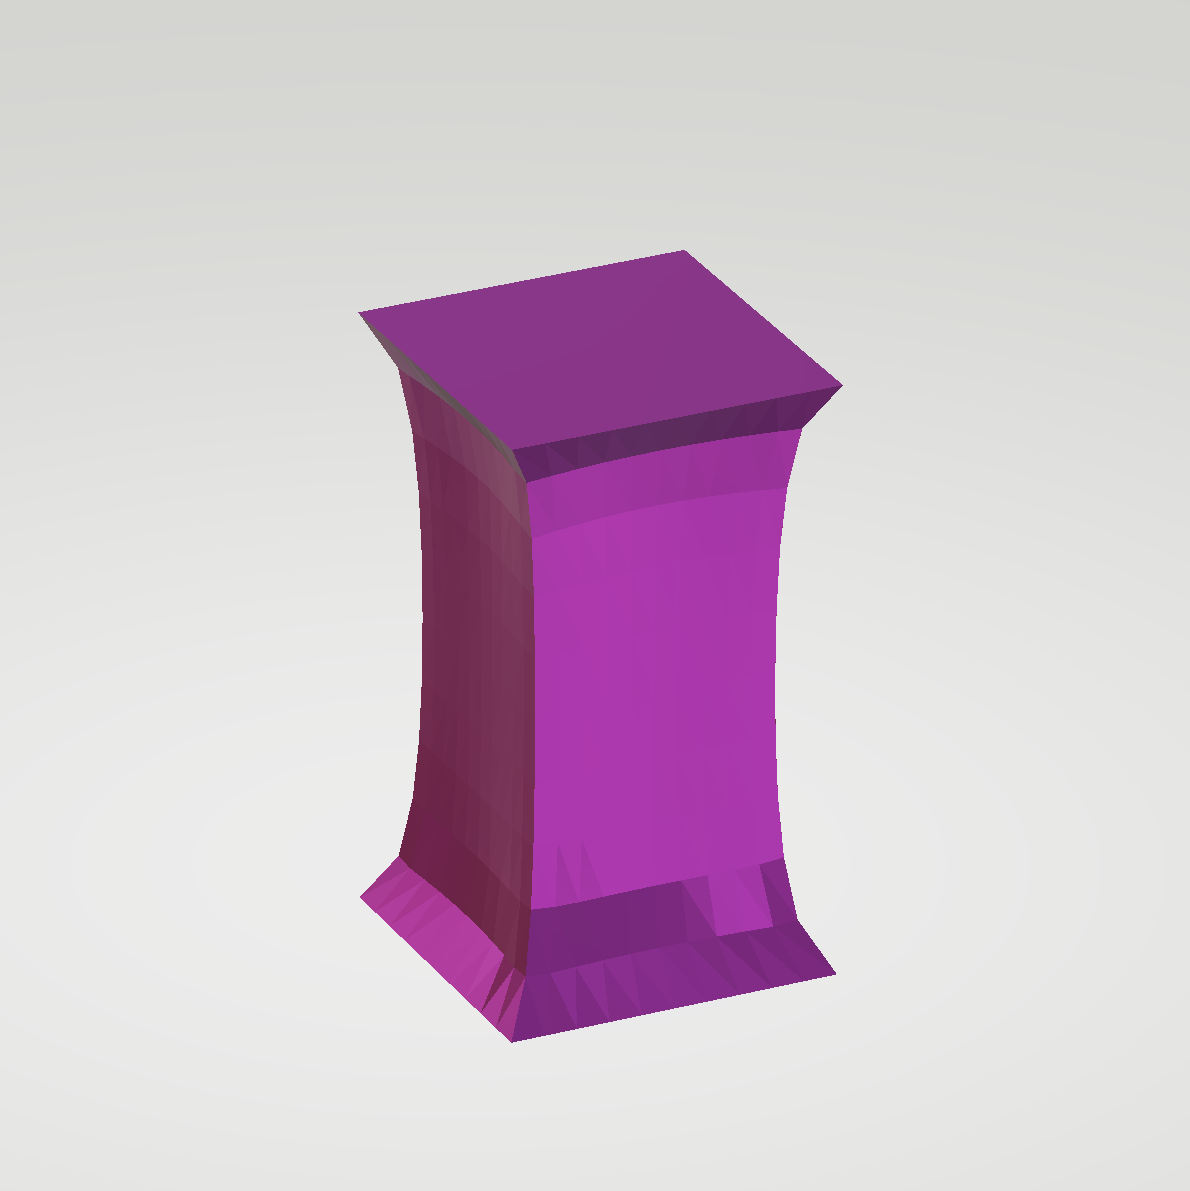
\includegraphics[width=0.24\textwidth]{resources/hexcli_step8.png}
        \hfill
        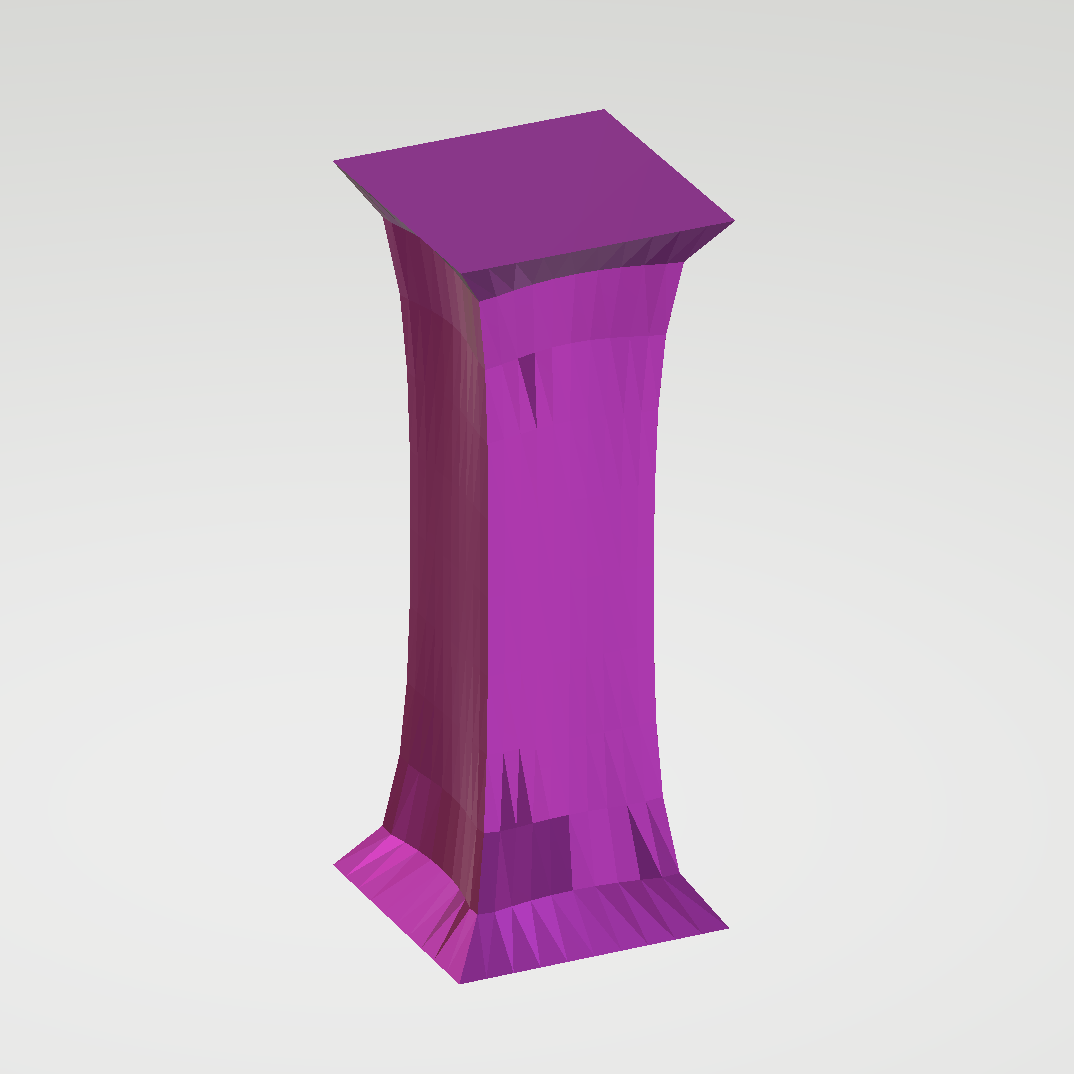
\includegraphics[width=0.24\textwidth]{resources/hexcli_step16.png}
        \hfill
        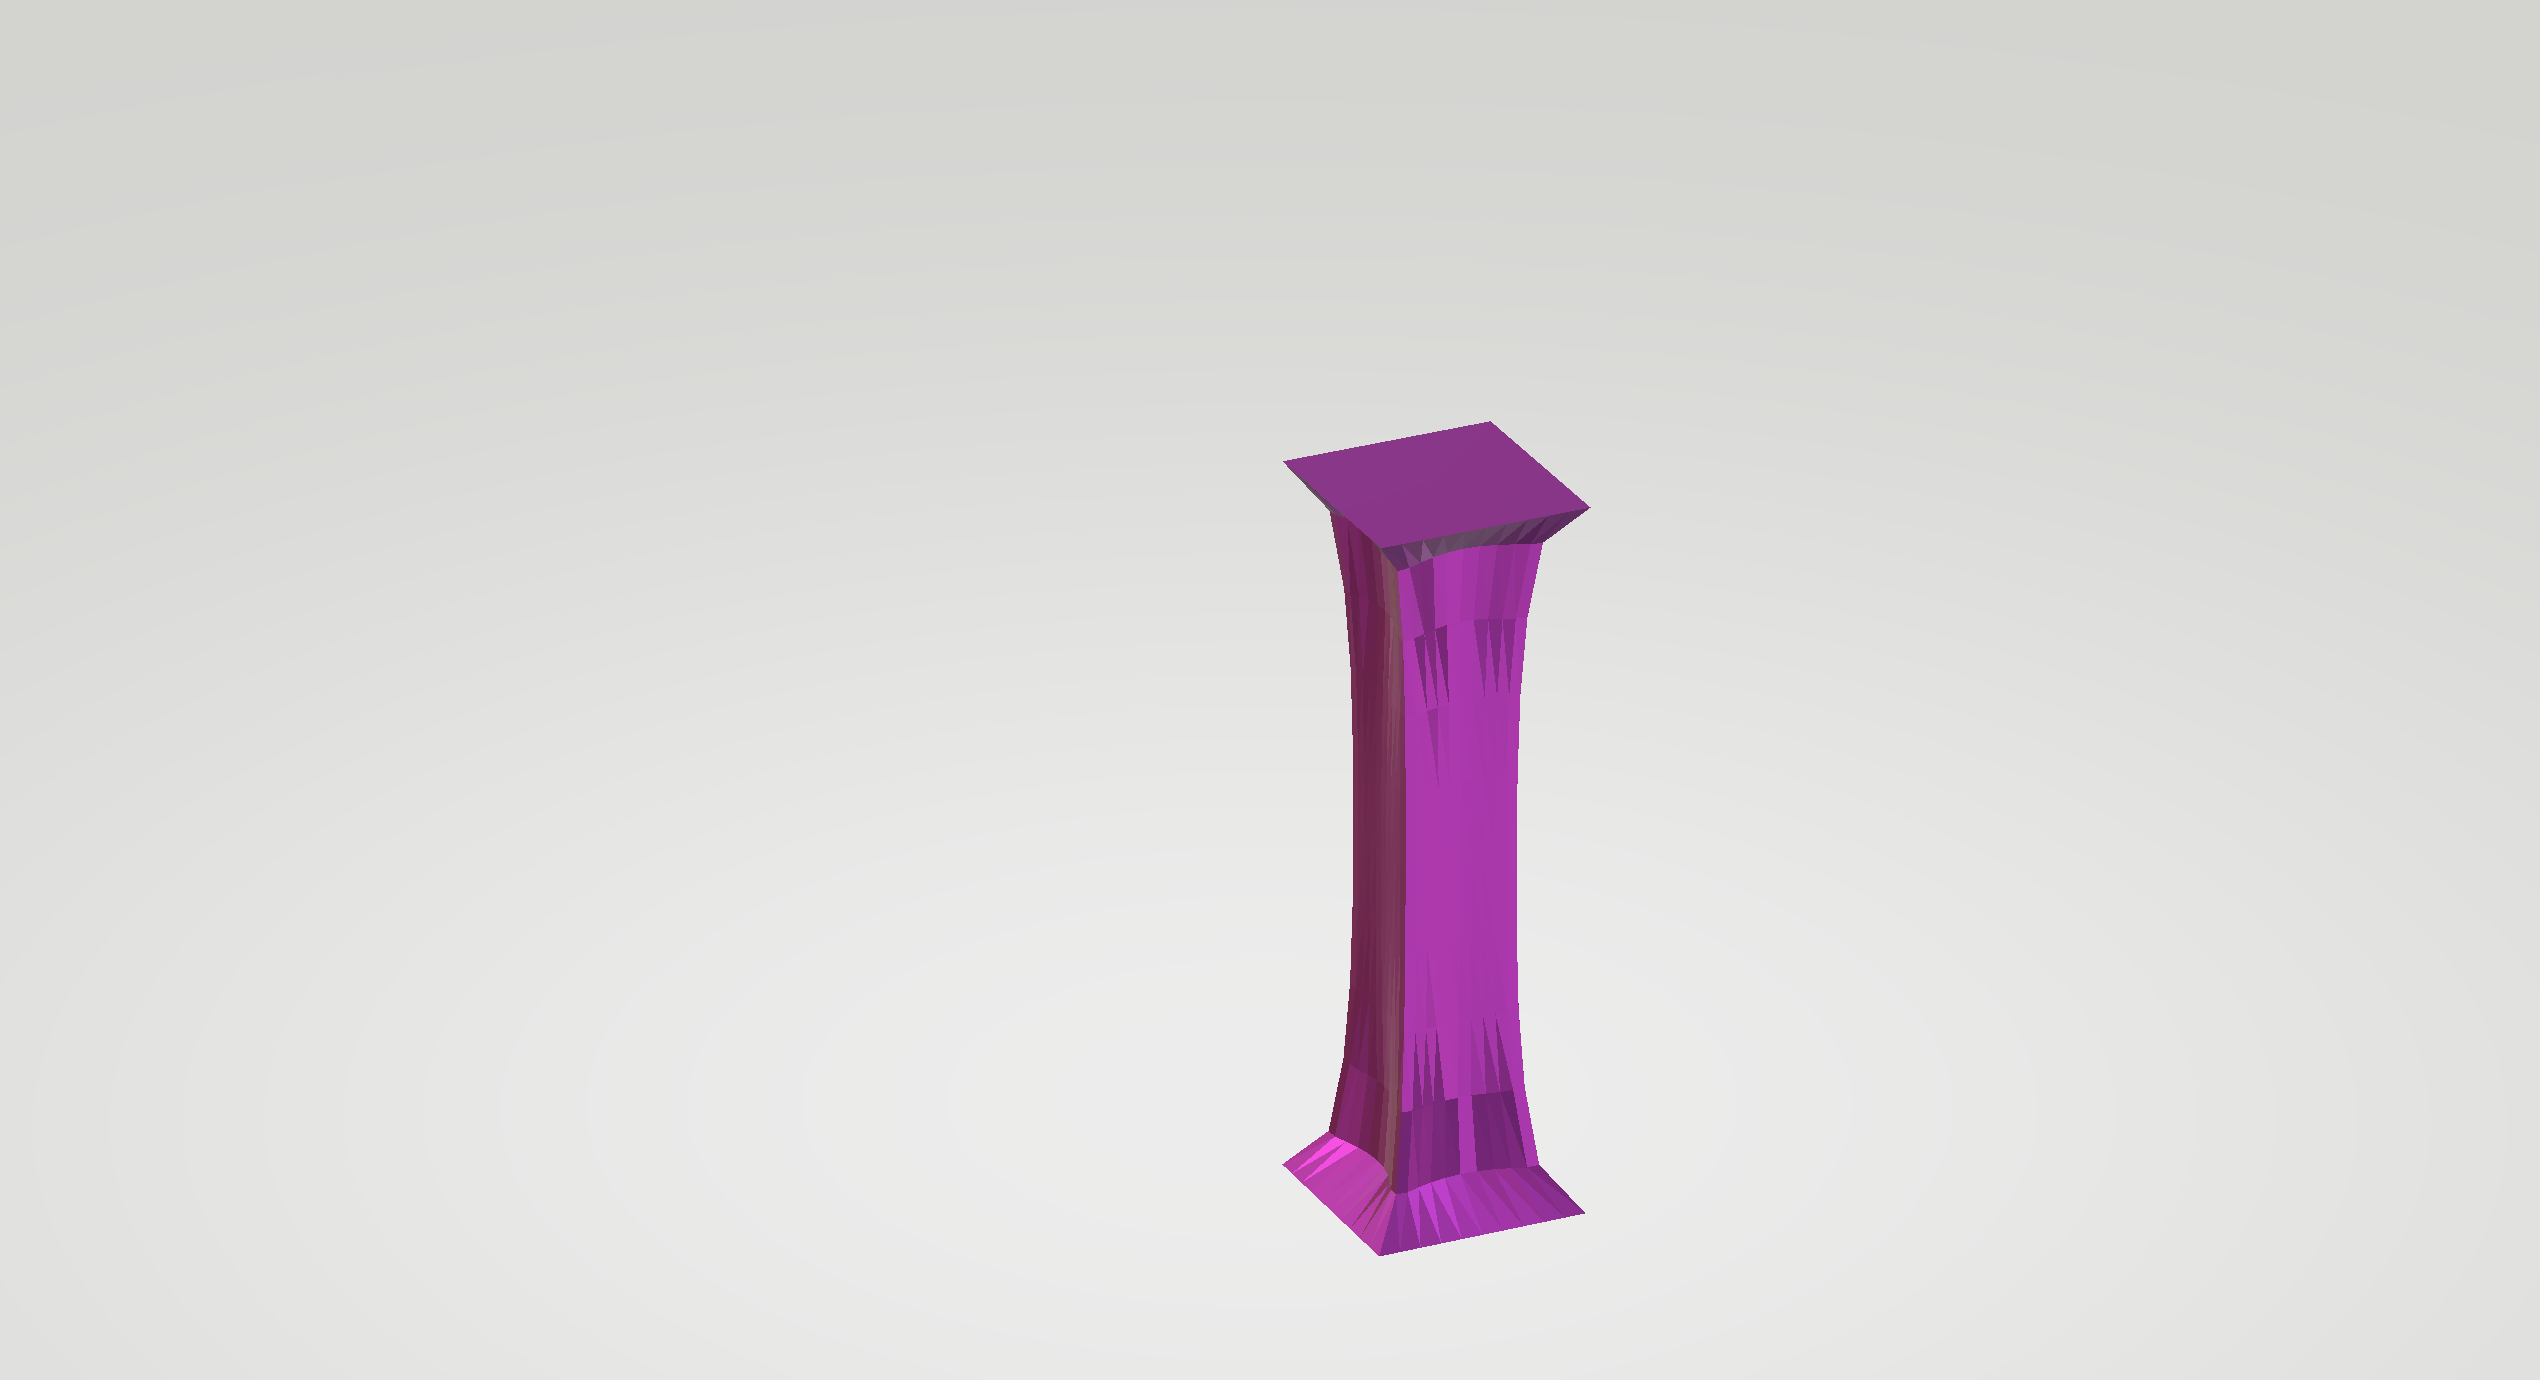
\includegraphics[width=0.24\textwidth]{resources/hexcli_step24.png}
        \caption{Stretch test on a hexahedral mesh}
    \end{subfigure}
    \vskip\baselineskip
    \begin{subfigure}[b]{\textwidth}
        \centering
        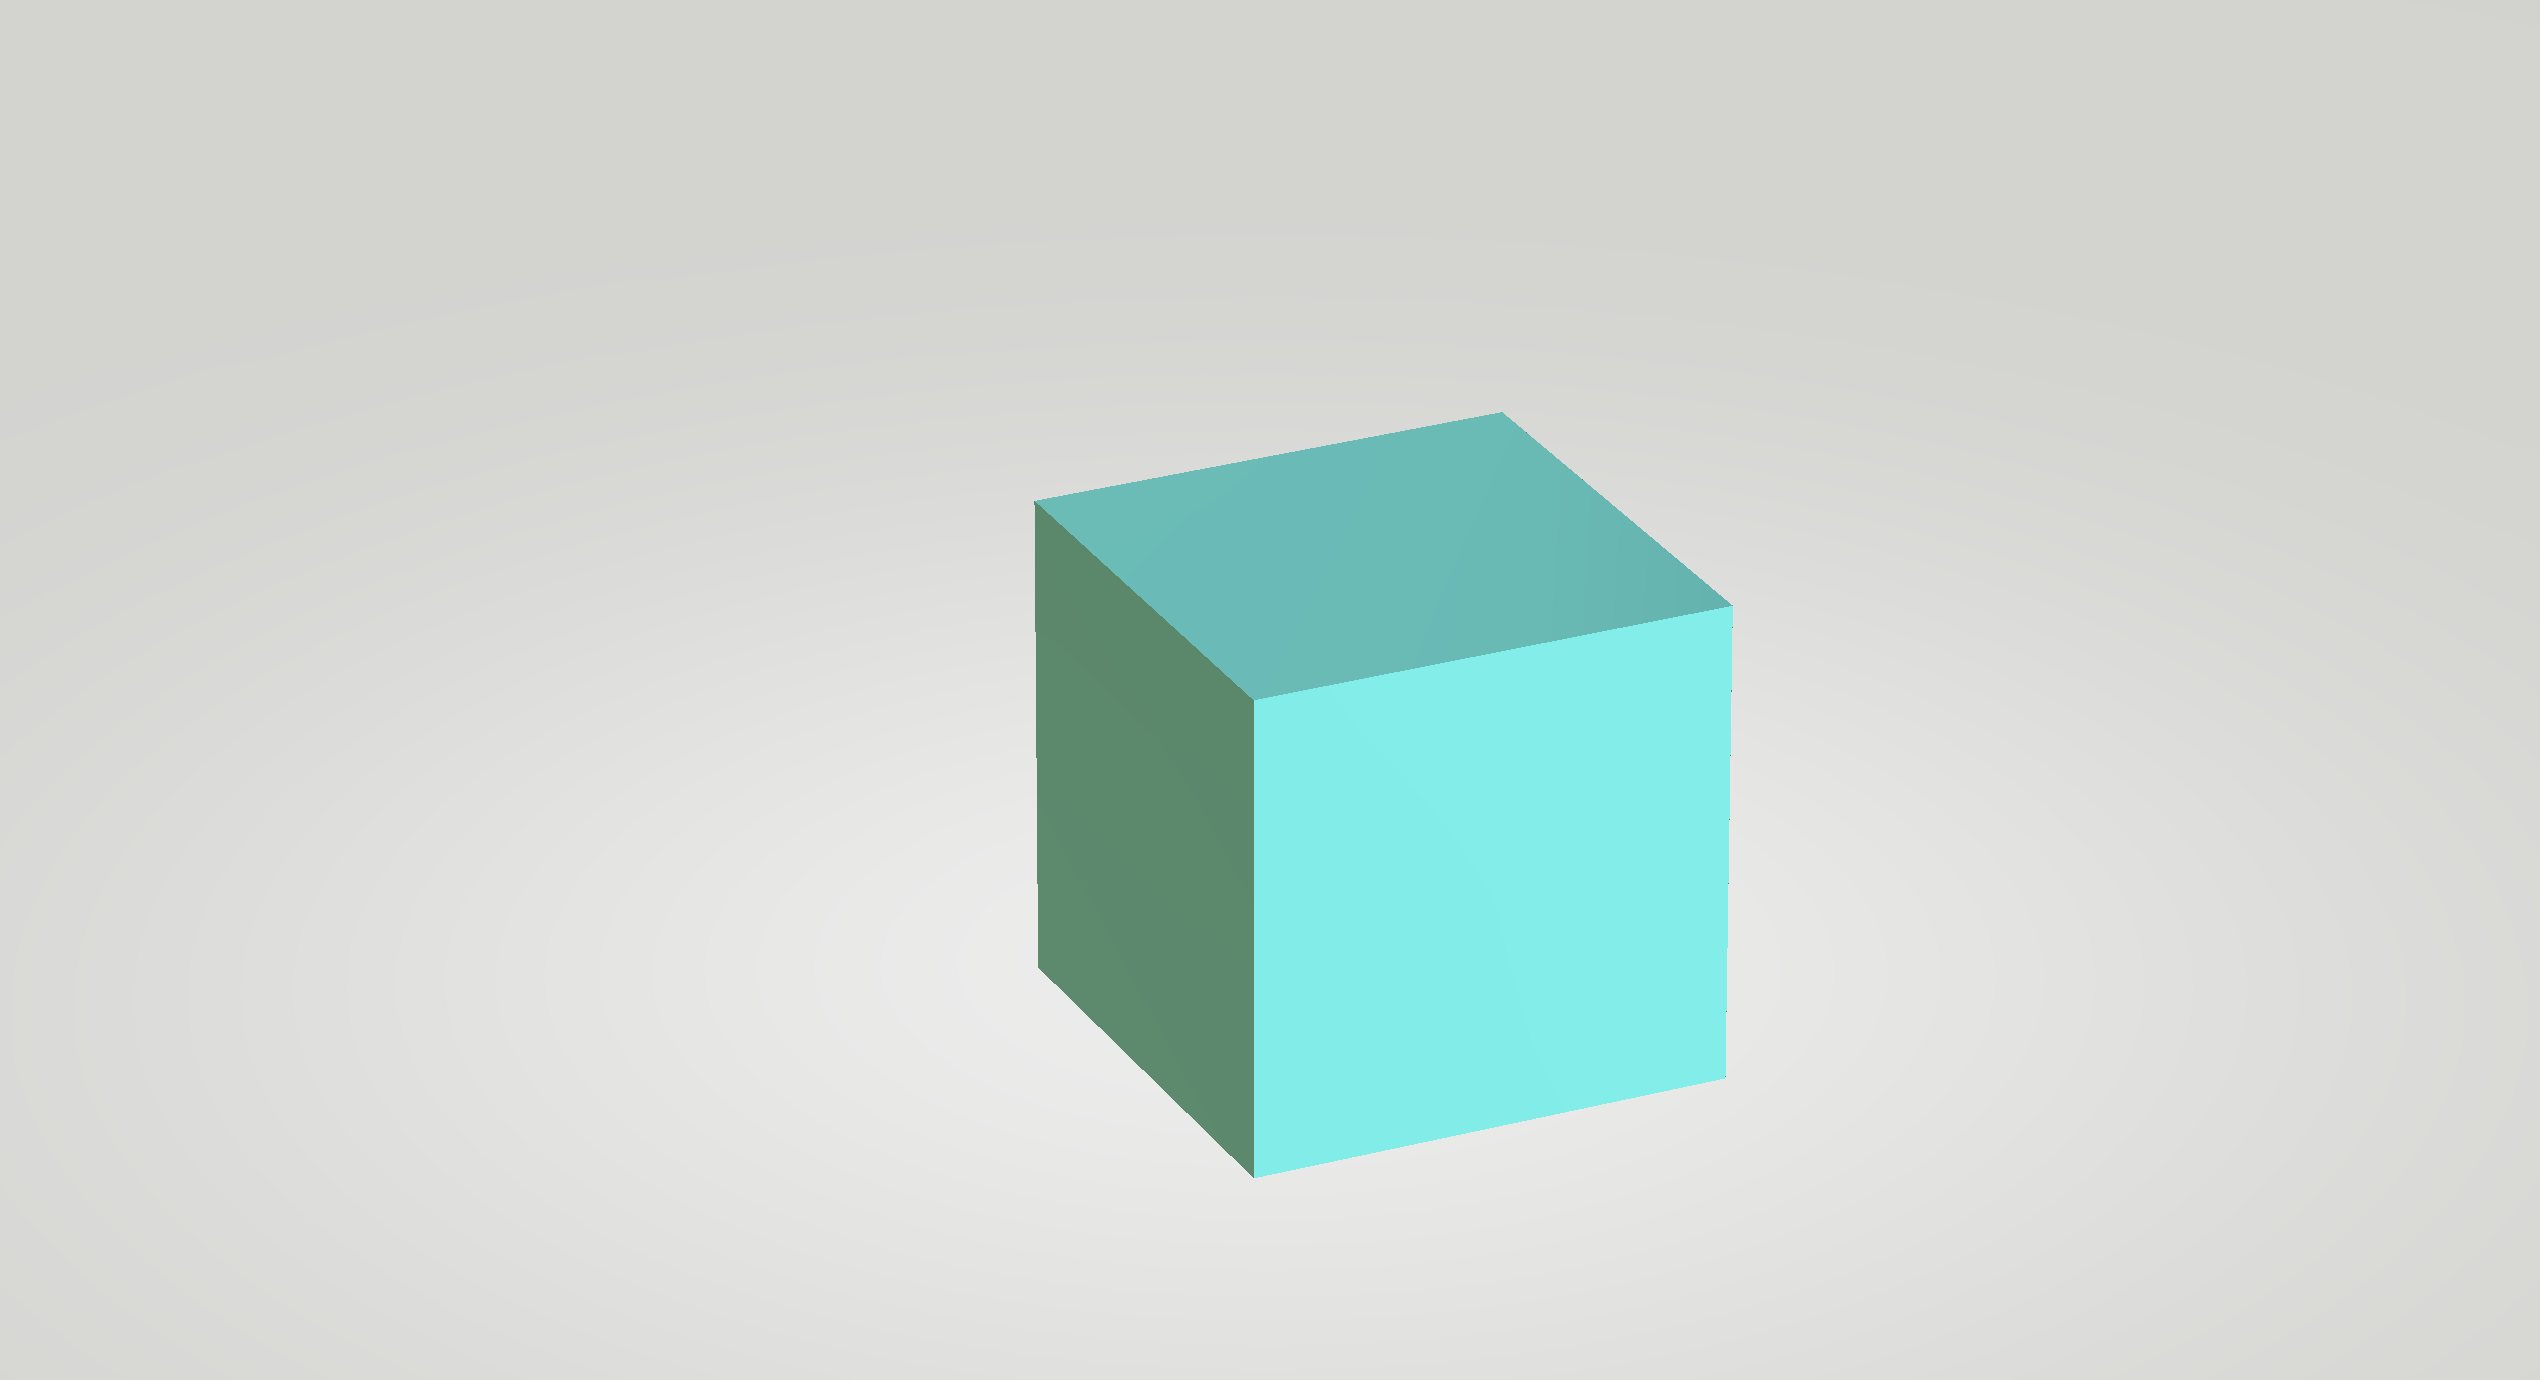
\includegraphics[width=0.24\textwidth]{resources/tetcli_step0.png}
        \hfill
        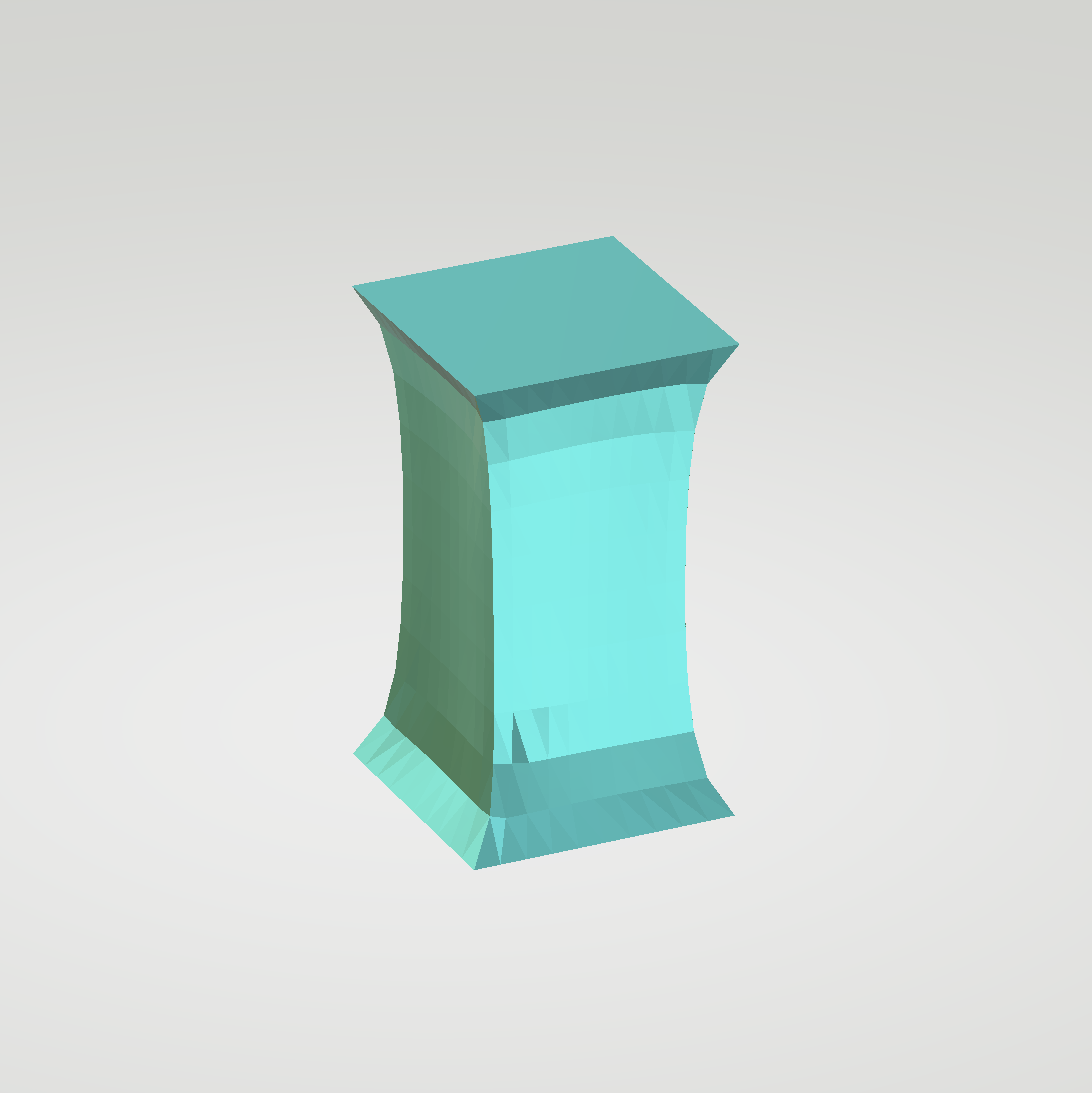
\includegraphics[width=0.24\textwidth]{resources/tetcli_step8.png}
        \hfill
        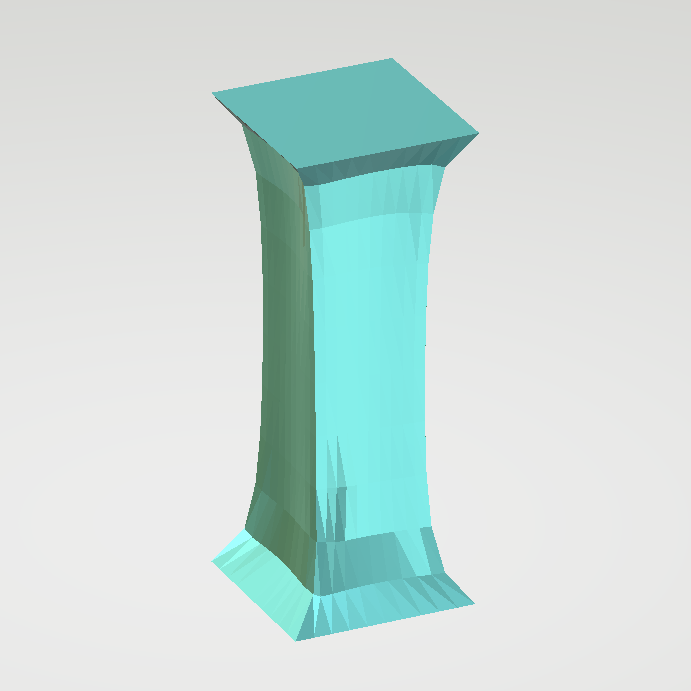
\includegraphics[width=0.24\textwidth]{resources/tetcli_step16.png}
        \hfill
        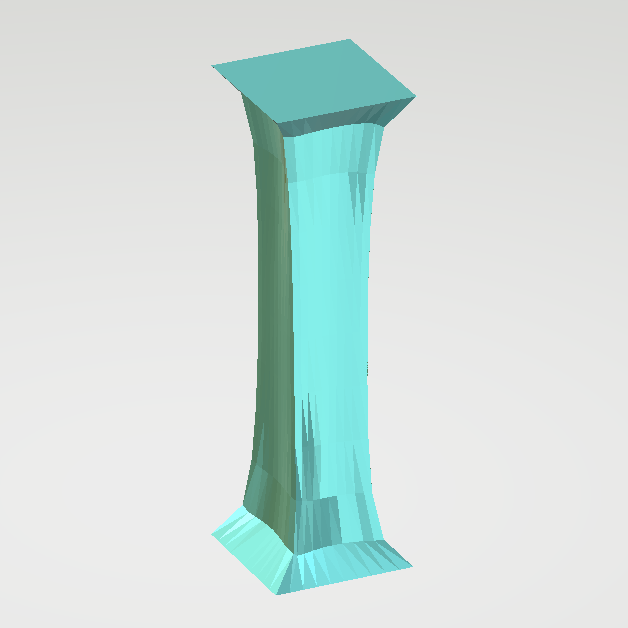
\includegraphics[width=0.24\textwidth]{resources/tetcli_step24.png}
        \caption{Stretch test on a tetrahedral mesh}
    \end{subfigure}
    \caption{Stretch test performed on a cube with (a) a hexahedral mesh and (b) a tetrahedral mesh}
    \label{fig:stretchtest}
\end{figure}





\section{Discussion}
Stuff, Taylor approx.


